\subsection{Describing the Metamodel}
\label{sec:dataset:architecture:metamodel}

% Conceptualise what we have in our workflow as a meta model.
% What are the components, and constraints? Discuss why we needed to add in constraints... Feedback from India

In the example above, we describe a basic model which was derived using information discovered from Argus' incremental development. In this section, we generalise this information and develop a metamodel from that model. This metamodel is represented as a \gls{uml} class diagram, shown in Figure~\ref{fig:dataset:metamodel_class_diagram}. A more extensive overview of the metamodel is provided in Appendix~\ref{ch:metamodel_class_diagrams}.

\begin{figure}[h]
  \centering
  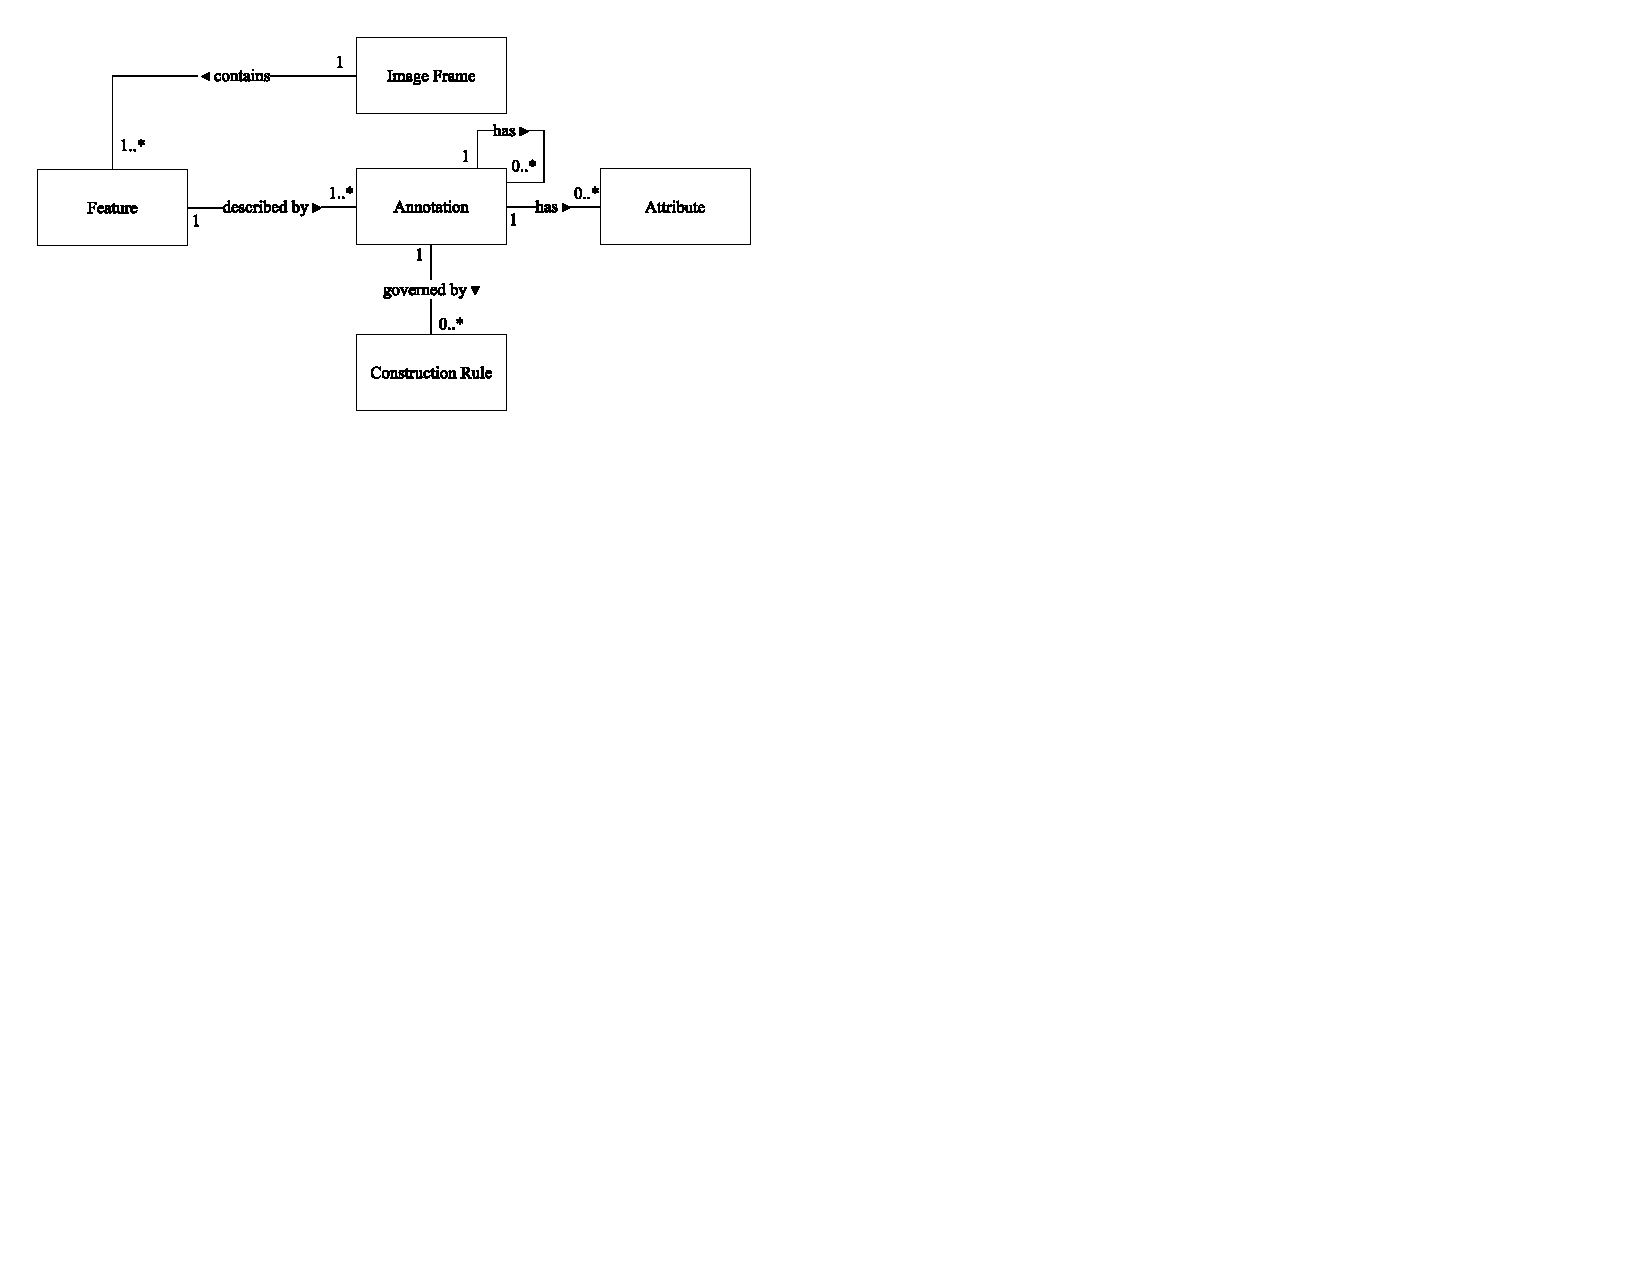
\includegraphics[width=\textwidth]{images/dataset/metamodel_class_diagram}
  \caption[Class diagram of our proposed metamodel]{A class diagram of our proposed metamodel.}
  \label{fig:dataset:metamodel_class_diagram}
\end{figure}

At the centre of this metamodel is an annotation, which (collectively) describe a feature within an image. Annotations may contain additional attributes to further extend what information they contain, and are governed by a set constrictions which we call `Construction Rules'.

These form layers of data within images that we annotate, which can be represented in a hierarchical data format (e.g., a tree) that describes the layering of a fully annotated photo's features.

We describe each of these classes in the following sections.

\paragraph{Image Frame}

An image frame is any visual representation of a graphic. We extend the possibilities of our metamodel beyond just static images---these frames may be those found in videos also.

\paragraph{Feature}

Image frames contain a certain number of features. These features are the key `concepts' within the image that we want to capture. There are two main features: (1) image-level features, and (2) segment-level features. Image-level features are those that apply to the entire frame and do not exist in a broken down context---we can't break down these features into their own subjects. This contrasts to segment-level features, which are features that only apply to a segmented region of the image. We identified four segment-level features in our example (all of which relate to one runner): Bib, Face, Prominence and Colours.

\paragraph{Annotation}

Annotations are simply a set of feature descriptors that describes what the feature is compromised of. From Table~\ref{tab:dataset:annotation_summary}, we describe a simple type system consisting of the following: \textit{Boolean}s, a restricted form of the \textit{Category} type (where possible values are $\{ \textsc{true}, \textsc{false} \}$); \textit{Polygon}s and \textit{Rectangle}s, generalised into a high-level \textit{Boundary} type; and \textit{Colour}s, represented as an RGB represented hexadecimal \textit{Label} (a generic labelling type). This only leaves our \textit{Collection} of runners: a data type which encompasses multiple annotations. Attributes can therefore be described by a relatively simple type system that is generalisable from \textit{Labels}, \textit{Boundaries}, \textit{Collections} and \textit{Categories}. We further develop this into a more extensive type tree (Figure~\ref{fig:metamodel_class_diagrams:annotation}).

\paragraph{Construction Rules} 

Construction Rules govern how attributes can be made. We break these down into four types: Dependencies, Conditions, Optionality and Restrictions (Figrue~\ref{fig:metamodel_class_diagrams:construction_rules}). Some annotations are dependent on others existing---these are rules that we name \textit{Dependencies}. For instance, we cannot annotate an \gls{rbn} if there is no $BibSheet$ annotated. Likewise, a $FaceBounds$ is dependent on where the $BibSheet$ is, and so the $BibSheet$ must be marked up first. These dependencies add order in which features are being extracted, which is important to the tagger marking up the photo. A \textit{Condition} is a construction rule that disallows a data tagger to create an annotation until a condition is met by the annotator. For instance, we can never have a $BibSheet$ above a $FaceBounds$, so when we can specify this as a condition. These are not bound to just geometric constraints; we also see that we cannot tag $Runners$ if the $PhotoCrowded$ annotation is marked as \textsc{true}. Not all annotations are needed---in these cases the annotation is restricted by an \textit{Optional} construction rule; by default, all annotations are required, but we can specify these to be optional using such a rule. Lastly, \textit{Restrictions} exist to prevent invalid data from being tagged. In our example, we implemented two restrictions in Argus: (1) a face region must be tagged within an aspect ratio of $3 \times BibSheet_{width} : 5 \times BibSheet_{height}$, and (2) the opposite edges of a face region must be at least 15 pixels apart. This helps prevent issues shown in Figure~\ref{fig:dataset:issues_with_tagging}.


\paragraph{Attributes}

Attributes exist to as a means capture further information about an annotation. We represent attributes in our metamodel as either implicit or explicit. As stated in Section~\ref{sec:dataset:architecture:what_to_capture}, those attributes which are required for the tagger to manually markup are explicit (i.e., manually must be added) whereas those that can be computed by the system are implicit (i.e., inferred from explicit attributes). A useful example of implicit attributes may be the bounding box and area that inferred from a polygon, both of which are key values required in training \glspl{nn}.